\section{A model for on-the-spot attention and response modulation support in online conversations}~\label{sec:design}
\subsection{An Intervention for Implicit Emotion Regulation}
The majority of research in digital emotion regulation has concentrated on explicit emotion regulation, which involves a conscious effort to change one's affective state. However, as per psychological research, implicit emotion regulation is also an essential component of overall well-being \cite{gyurak2011explicit}, \cite{braunstein2017explicit}. While explicit emotion regulation requires conscious effort to initiate and monitor during implementation and is associated with some level of insight and awareness, implicit emotion regulation is elicited automatically by the stimulus itself and runs to completion without monitoring and can occur without insight and awareness. Habitual emotion modification, in which a person performs emotion regulation to routinely achieve a specific goal, is an example of implicit emotion regulation \cite{gross2006emotion}. 
Currently, the digital tools available to assist ER are based on the user's need; thus, they not only require their users to be aware that they are attempting to change their affective state but also to choose appropriate tools to do so. Scrolling through social media applications to escape participating in a situation is one such example of digital emotion regulation where the user is although habitually scrolling but is aware of the platform. As a result, we believe that by emphasising instances of intense emotional expression and reactions, we can make emotionally charged elements clear and easy to perceive, which, when encountered repeatedly, will trigger habitual emotion regulation.
\begin{figure}[h]
  
    \centering
    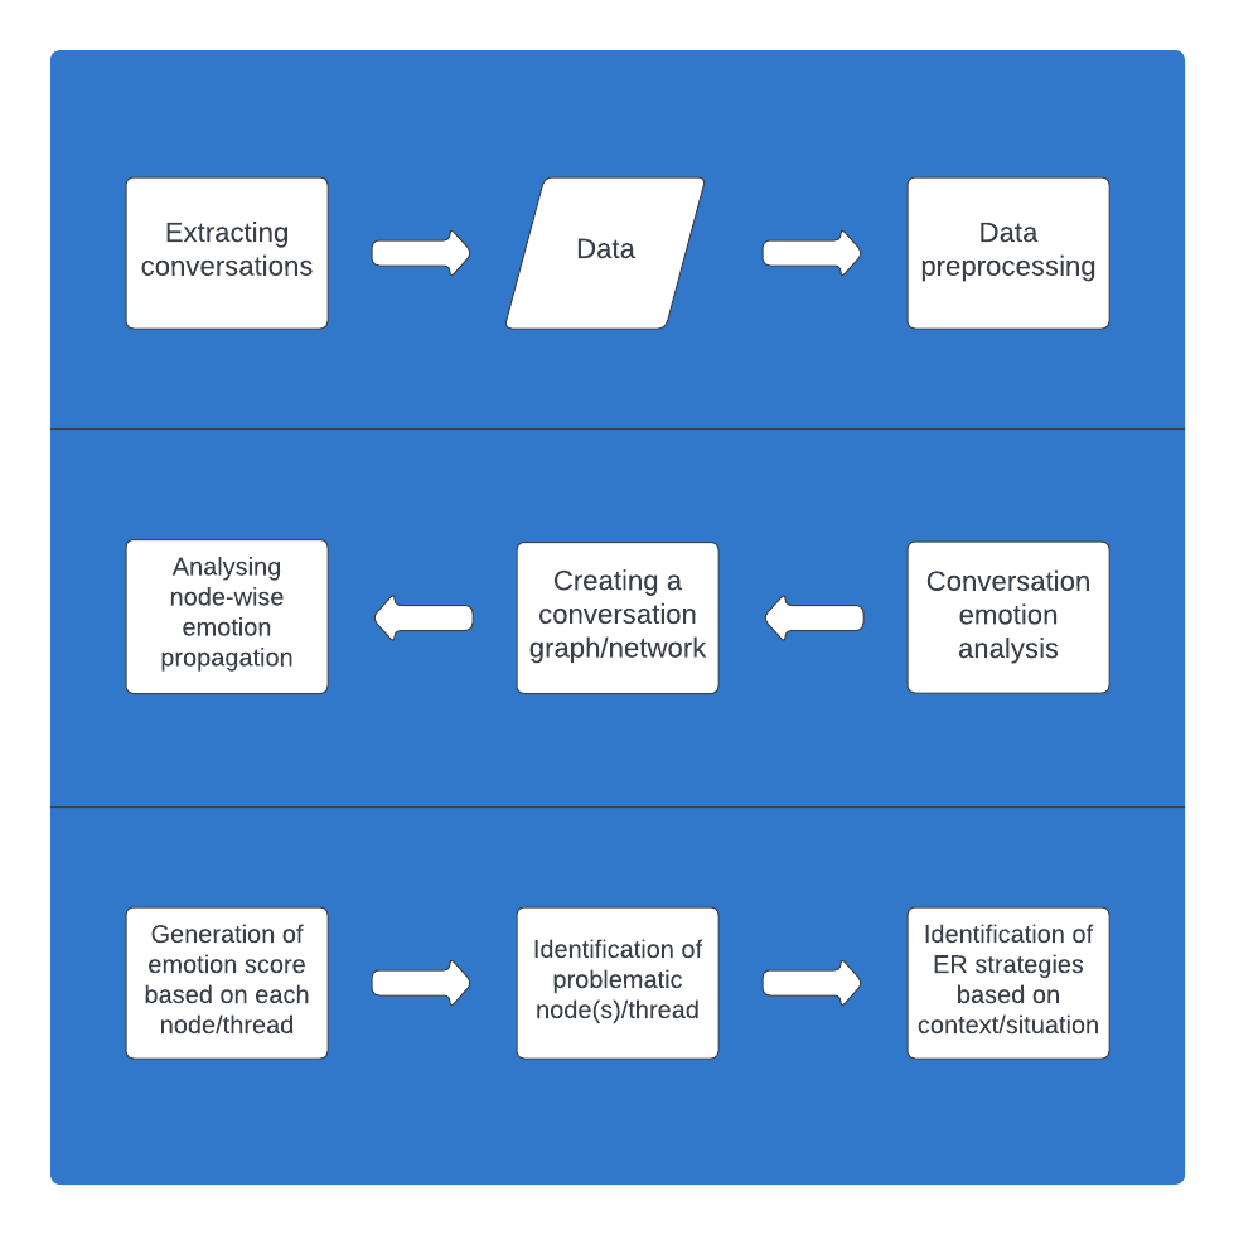
\includegraphics[width=12cm,height=12cm,keepaspectratio]{framework.pdf}
%   \includegraphics[width=5cm,height=5cm,keepaspectratio]{samples/sample_convv.png}
%   \includegraphics[width=5cm,height=5cm,keepaspectratio]{samples/sample_conv_graphh.png}
  \caption{Framework for encouraging on-spot emotion regulation in social media conversations}
  \label{fig:Framework}
  \end{figure} 
\subsection{Proposed methodology}
The proposed framework for encouraging emotion regulation in social media conversations is depicted in Figure-\ref{fig:Framework}. It is composed of three key components: data retrieval, emotion propagation analysis, and emotion regulation recommendations. The data retrieval process starts with gathering information from social media conversations, in this case Twitter conversations. In recent years, Twitter has been a popular destination for hashtag-based social movements such as \#MeToo and \#BlackLivesMatter, but the platform's free speech policy also increases the risk of hate and harassment. Therefore, we gathered a variety of Twitter conversations and saved them as CSV files. We used feature engineering to create a set of files, each containing a conversation wherein each row comprised of a text string representing a tweet or a comment, as well as their ID and metadata (parameters like the number of comments received, authors who replied etc). The second component then analyses emotion propagation using these CSV files. It begins with categorising the emotions expressed in tweets. Emotions are divided into 6 primary and 27 secondary groups. We use the primary emotion categories in this work to classify the emotion in tweets. We generate a graph (G) of the conversation after classifying the tweets into 6 emotion classes. This graph is used to calculate the emotional impact (given by Equation 1) of individual tweets on the entire conversation as well as the percentage distribution of various emotions in the discussion. 
The conversation graph G can be defined as:


\textit{\textbf{G = (V, E, A)}, where V is the set of nodes, E is the set of edges representing the nodes' existing relations, and A denotes the set of attribute vectors. The value of n=|V| represents the total number of vertices, m=|E| represents the total number of edges, and A (A1, A2, A3... Ak) associates with nodes in V and describes their characteristics, where k is the number of attributes each node has.}



The impact of nodes in G = (V, E, A) on the root node R is given by:
\begin{equation}
\forall \,V \in G-\{R\},
E_{m}(R) = \sum{E_{m}(V1, V2, V3....Vn)}
\end{equation}
where:
\begin{conditions}
E_{m}(Vi) & f(Ai)
\end{conditions}
Following that, in the final component, we use the graph to identify the nodes that have the greatest impact on the emotion of the conversation and apply this information to identify scenarios where emotion regulation needs to be undertaken and offer support for the same.
 
%%%%%%%%%%%%%%%%%%%
\begin{figure*}[h]
  \begin{minipage}{.33\textwidth}
    \centering
    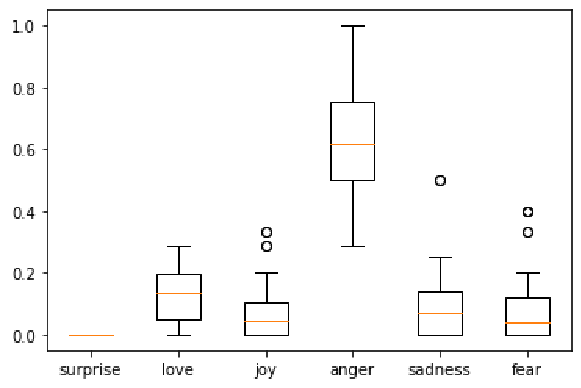
\includegraphics[width=5cm,height=5cm,keepaspectratio]{download.pdf}
    \subcaption{Dominant Emotion: Anger}
  \end{minipage}%
  \begin{minipage}{.33\textwidth}
    \centering
    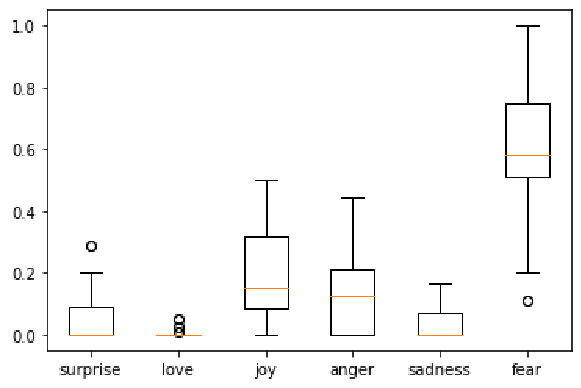
\includegraphics[width=5cm,height=5cm,keepaspectratio]{fear_wie.pdf}
    \subcaption{Dominant Emotion: Fear}
  \end{minipage}%
  \begin{minipage}{.33\textwidth}
    \centering
    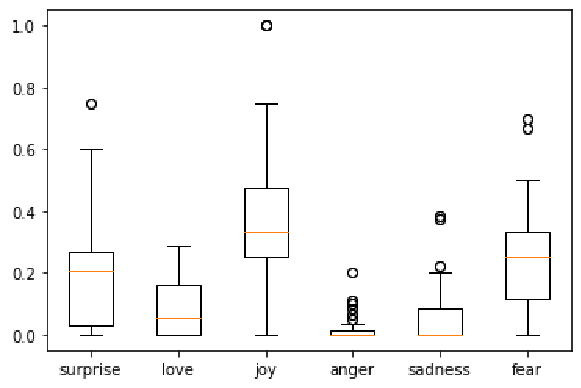
\includegraphics[width=5cm,height=5cm,keepaspectratio]{joy.pdf}
    \subcaption{Dominant Emotion: Joy}
  \end{minipage}
 \medskip
  \begin{minipage}{.5\textwidth}
    \centering
    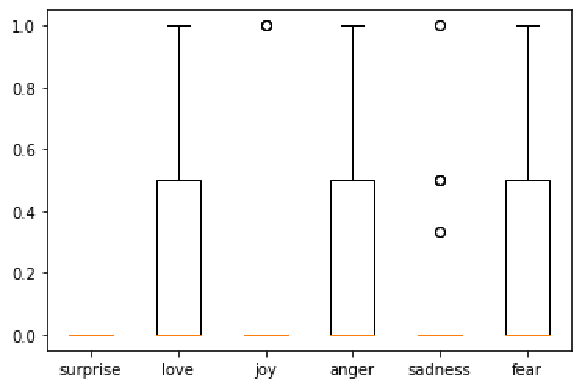
\includegraphics[width=5cm,height=5cm,keepaspectratio]{love_wie.pdf}
    \subcaption{Dominant Emotion: Love}
  \end{minipage}%
  \begin{minipage}{.5\textwidth}
    \centering
    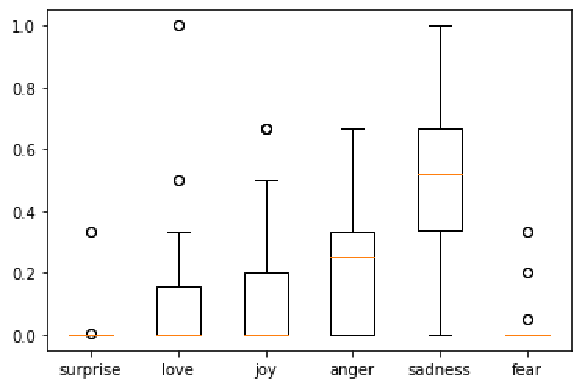
\includegraphics[width=5cm,height=5cm,keepaspectratio]{sad_wie.pdf}
    \subcaption{Dominant Emotion: Sadness}
  \end{minipage}
  
%   \includegraphics[width=5cm,height=5cm,keepaspectratio]{samples/sample_convv.png}
%   \includegraphics[width=5cm,height=5cm,keepaspectratio]{samples/sample_conv_graphh.png}
  \caption{Percentage distribution of emotions in the reply tree of influential nodes of conversations where the dominant emotion is (a) Anger (b) Fear (c) Joy (d) Love and (e) Sadness}
  \label{SampleConv}
  \end{figure*}
\subsection{Experimental Evaluation and Analysis}
The structure and toxicity of Twitter conversations have been extensively researched. We use the findings from literature to validate the applicability of our framework. We do so based on three attributes: structural characteristics, emotions and virality, and the development of connective action.  It was observed that the toxicity of a reply tree increases with its size, width, and density. The percentage of angry tweet responses skyrockets at 40\% and continues to rise until it reaches 80\% (Figure-\ref{SampleConv} (a)). Because anger spreads faster than other emotions, the same pattern can be seen when comparing the percentage of emotions contained in the nodes. After identifying the conversation graph's influential nodes, we calculated their Wiener index with respect to the percentage of emotions contained in their reply trees. It was discovered that the Wiener index for anger tends to increase the most. It begins low and starts to rise as the percentage of anger in the reply tree increases. It peaks at 60\% anger in the reply tree nodes and then drops by a small value before plateauing at the end. This leads us to the conclusion that the influential node initially broadcasts a variety of emotions, and as the size of its reply tree and the percentage of anger grows, it transforms into a viral spread in which the nodes of this reply tree receive more back-and-forth engagement. 

When the user activity in the influential nodes was examined, it was discovered that the number of responses received by a tweet is directly proportional to the amount of emotion contained in the tweet. Although tweets expressing anger and love received the most responses, the majority of these responses were angry. Furthermore, tweets expressing love received the angriest or rage-inducing responses.

\begin{table}[h]
\caption{Comparison of proposed framework against Perspective API \cite{bworld}}
\label{tab:my-table}
\resizebox{\columnwidth}{!}{%
\begin{tabular}{llll}
\hline
Utilised Model &
  \begin{tabular}[c]{@{}l@{}}Identification of\\ influential nodes\end{tabular} &
  \begin{tabular}[c]{@{}l@{}}Percentage of nodes\\  identified as toxic\end{tabular} &
  \begin{tabular}[c]{@{}l@{}}Possible reduction in\\ toxicity if acted on\\ these nodes\end{tabular} \\ \hline
Proposed Framework &
  \begin{tabular}[c]{@{}l@{}}Based on\\ impact score,\\ taking into account\\ the tweet text \\ as well as its\\ connectivity\end{tabular} &
  1-4\% &
  10\% \\ \hline
Perspective API \cite{bworld} &
  \begin{tabular}[c]{@{}l@{}}Based on\\ toxicity, taking \\ into account only\\ the tweet text\end{tabular} &
  1-2\% &
  7\% \\ \hline
Combination &
  \begin{tabular}[c]{@{}l@{}}Takes into account \\ the emotion in the\\ tweet text, the \\ connectivity\\ as well as its toxicity\end{tabular} &
  1-4\% &
  12\% \\ \hline
\end{tabular}%
}
\end{table}

Aside from preventing the compounding of anger or hate speech in general that later becomes toxic, this framework considers the subjectivity of toxicity by not relying solely on the content of a post/reply/comment and considering its impact on the ongoing conversation. We evaluated our framework by comparing it to the toxicity scores generated by the Google Perspective API \cite{bworld} as shown in Table-\ref{tab:my-table}. The Perspective API provides information about a comment's potential impact on a conversation by assigning a "toxicity" score to it. When the toxicity of the conversation was examined, it was discovered that not only were the most toxic tweets/comments also some of the influential nodes but that more than 87\% of the toxicity of the overall conversation was concentrated in the reply tree of influential nodes. We used the toxicity score from the Perspective API \cite{bworld} to find the influential nodes because the goal is to reduce the induction of hate speech in a conversation by analysing its influential nodes. Thereafter, we used a combination of our rule and toxicity scores to identify influential nodes in a conversation. We discovered that while the influential nodes generated by our framework and the Perspective API have a 75\% match, the influential nodes generated by the combination of the framework and the API have a 94.3\% match. 
This confirms that the proposed framework can be used to identify comments that may be contributing to the toxicity of a post while taking into account their subjectivity and whether or not they are individually toxic.
We also discovered that, while our model could reduce hate speech by 10\% and the Perspective API by 7\%, the combination of our model and the API could reduce toxicity by 12\%.
 

